\documentclass{amsart}

\usepackage{amsfonts,amssymb,amscd,amsmath,enumerate,verbatim, calc,xypic, appendix, tikz, float}
\usepackage{graphicx, chngpage, mathtools,longtable, listings}
\usepackage{hyperref}
\hypersetup{pdfborder=0 0 0}

\usetikzlibrary{fit, arrows, automata}

\graphicspath{{./images/}} \tolerance=1000 \CompileMatrices
\newcommand{\centered}[1]{\begin{tabular}{l} #1 \end{tabular}}



\newcommand{\sss}{\scriptscriptstyle}
\newcommand{\ges}{\operatorname{\sss\geqslant}}
\newcommand{\les}{\operatorname{\sss\leqslant}}
\newcommand{\sges}{\operatorname{\sss>}}
\newcommand{\sles}{\operatorname{\sss<}} \newcommand{\maxi}{\operatorname
{\max}} \newcommand{\cls}[1]{{\operatorname{cls}(#1)}}
\newcommand{\col}{\colon}
\newcommand{\dd}{\partial}
\newcommand{\HH}[2]{\operatorname{H}_{#1}(#2)}
\newcommand{\Ker}{\operatorname{Ker}} \newcommand{\Coker}{\operatorname{Coker}}
\newcommand{\ds}{\operatorname{\displaystyle}}
\newcommand{\chr}{\operatorname{char}}
\newcommand{\la}{\operatorname{\!\langle\!}}
\newcommand{\lra}{\longrightarrow}
\newcommand{\pd}[2]{\operatorname{pd}_{#1}{#2}}
\newcommand{\rank}{\operatorname{rank}} \newcommand{\Hom}{\operatorname{Hom}}
\newcommand{\Gdim}[2]{\operatorname{G-dim}_{#1}{#2}}
\newcommand{\Hdim}[2]{{\operatorname{G}{\!}^*{\!}\operatorname{-dim}_{#1}{#2}}}
\newcommand{\Cdim}[2]{\operatorname{CI-dim}_{#1}{#2}}
\newcommand{\PCIdim}[2]{{\operatorname{CI}{\!}_*{\!}\operatorname{-dim}_{#1}{#2}}}
\newcommand{\CMdim}[2]{\operatorname{CM-dim}_{#1}{#2}}
\newcommand{\hdim}[2]{\operatorname{H-dim}_{#1}{#2}}
\newcommand{\Pdim}[2]{\operatorname{P-dim}_{#1}{#2}}
\newcommand{\Tor}[4]{\operatorname{Tor}_{#1}^{#2}(#3,#4){}}
\newcommand{\Ext}[4]{\operatorname{Ext}_{#1}^{#2}(#3,#4){}}
\newcommand{\var}{{\hskip1pt\vert\hskip1pt}}
\newcommand{\depth}[2]{\operatorname{depth}_{#1}{#2}}
\newcommand{\edim}{\operatorname{edim}}
\newcommand{\codepth}{\operatorname{codepth}}
\newcommand{\dime}{\operatorname{dim}}
\newcommand{\grade}[2]{\operatorname{grade}_{#1}{#2}}
\newcommand{\xra}{\xrightarrow}
\newcommand{\cx}[2]{\operatorname{cx}_{#1}{#2}}
\newcommand{\infe}{\operatorname{inf}} \newcommand{\supr}{\operatorname{sup}}
\newcommand{\card}{\operatorname{card}} \newcommand{\Supp}[2]{\operatorname
{Supp}_{#1}{(#2)}} \newcommand{\ann}{\operatorname{ann}}
\newcommand{\syz}[3]{\operatorname{Syz}_{#1}^{#2}{(#3)}}
\newcommand{\ba}{{\boldsymbol a}} \newcommand{\bX}{{\boldsymbol X}}
\newcommand{\bB}{{\boldsymbol B}} \newcommand{\bC}{{\boldsymbol C}}
\newcommand{\bF}{{\boldsymbol F}} \newcommand{\BF}{{\mathbb F}}
\newcommand{\BN}{{\mathbb N}} \newcommand{\BZ}{{\mathbb Z}}
\newcommand{\bsb}{{\boldsymbol b}} \newcommand{\bsy}{{\boldsymbol y}}
\newcommand{\bsf}{{\boldsymbol f}} \newcommand{\bsm}{{\boldsymbol m}}
\newcommand{\bsn}{{\boldsymbol n}} \newcommand{\bsp}{{\boldsymbol p}}
\newcommand{\bsq}{{\boldsymbol q}} \newcommand{\bss}{{\boldsymbol s}}
\newcommand{\bsx}{{\boldsymbol x}}
\newcommand{\E}[2]{\operatorname{E}^{#1}_{#2}} \newcommand{\im}{\operatorname
{Im}} \newcommand{\md}{{\displaystyle}}
\newcommand*\conj[1]{\bar{#1}}

\newtheorem{theorem*}{Main Theorem}

\newtheorem{theorem}{Theorem}[section]
\theoremstyle{theorem}
\theoremstyle{theorem*}
\newtheorem{corollary}[theorem]{Corollary}
\newtheorem{lemma}[theorem]{Lemma}
\newtheorem{proposition}[theorem]{Proposition}
\newtheorem{question}[theorem]{Question}
\newtheorem{partt}{Part}
\theoremstyle{definition}
\newtheorem{chunk}[theorem]{}
\newtheorem{schunk}[theorem]{}
\newtheorem{example}[theorem]{Example}
\newtheorem{examples}[theorem]{Examples}
\newtheorem{remark}[theorem]{Remark}
\newtheorem{computation}[theorem]{Computation}
\newtheorem{notation}[theorem]{Notation}
\newtheorem{definition}{Definition}
\begin{document}

\date{\today}
\title[Euler Matrices and Mahler Measure] {Euler Matrices of Quivers and Mahler Measure}
\author[T. Nichols]{Ty Nichols}
\address{Department of Mathematics, Northeastern University, Boston,
    Massachusetts~02115}
\email{nichols.t@northeastern.edu}
\begin{abstract} For a given quiver $Q$, we can define the matrix $B$ such that
    $B = -(E^T)E^{-1}$, where $E$ is the Euler matrix of $Q$. We investigate
    the roots of the characteristic polynomial of $B$ for
    small quivers, including the simply laced Dynkin diagrams. We show that 
    the characteristic polynomial of $B$ is reciprocal and that its roots must
    lie on the unit circle in the complex plane when $E + E^T$ is positive definite.
    For this project, we consulted with Professor Harm Derksen. 
\end{abstract}
\maketitle

\section{Introduction}

We investigate the properties of polynomials formed by the matrix $B$ defined
on a quiver (see sections 1.1-1.5). In particular, we ask these questions:

\begin{question}
    Which polynomials $P$ can be written as the characteristic polynomial of a 
    matrix $B$ for some Euler Matrix $E$ of a quiver?
\end{question}

\begin{question}
    Given two quivers $Q$ and $Q'$, if $Q$ is a subgraph of $Q'$, is $M(Q) \leq
        M(Q')$?
\end{question}

\begin{question}
    Given a triangular matrix $E$, is it the case that if $E + E^T$ is positive semidefinite,
    then the characteristic polynomial of $B$ has roots on the unit circle in the complex plane?
\end{question}

We now introduce basic terminology that motivates our approach to the
problem. The main objects under study are quivers, and the related matrices are
defined for use in the theory of quiver representations.

\subsection{Quivers}

\begin{definition} \cite{dw} A \textit{quiver} $Q$ is a 4-tuple $Q = (Q_0, Q_1,
        h, t)$ where $Q_0$ is a finite set of vertices, $Q_1$ is the set of
    edges, and $h: Q_1 \rightarrow Q_0$ and $t : Q_1 \rightarrow Q_0$ are
    functions that give the head and tail of each edge, respectively.
\end{definition}

\begin{definition} \cite{dw} A \textit{path} on a quiver $Q = (Q_0, Q_1, h, t)$
    from $u$ to $v$ for $u, v \in Q_0$ is some sequence of edges $e_0, \dots
        e_n$ such that for $0 \leq i \leq n$, $h(e_{i-1}) = t(e_i)$ and $t(e_0) =
        u$, $h(e_n) = v$.
\end{definition}

\begin{example}
    Consider the quiver illustrated by the following diagram:

    $$
        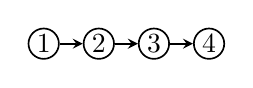
\begin{tikzpicture}[
                > = stealth, % arrow head style
                % shorten > = 1pt, % don't touch arrow head to node
                auto,
                node distance = 7mm, % distance between nodes
                semithick % line style
            ]

            \tikzstyle{every node}=[
            draw = black,
            circle,
            inner sep = 1pt,
            minimum size = 0.1mm
            ]

            \node (1) {$1$};
            \node (2) [right of=1] {$2$};
            \node (3) [right of=2] {$3$};
            \node (4) [right of=3] {$4$};

            \path[->] (1) edge (2);
            \path[->] (2) edge (3);
            \path[->] (3) edge (4);
        \end{tikzpicture}
    $$

    Then $Q_0 = \{1, 2, 3, 4\}$, $Q_1 = \{(1,2), (2,3), (3,4) \}$, and $h((1,2))
        = 2$ while $t((1,2)) = 1$.
\end{example}

\begin{example}
    Consider

    $$
        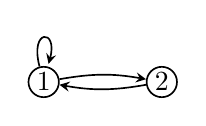
\begin{tikzpicture}[
                > = stealth, % arrow head style
                % shorten > = 1pt, % don't touch arrow head to node
                auto,
                node distance = 15mm, % distance between nodes
                semithick % line style
            ]

            \tikzstyle{every node}=[
            draw = black,
            circle,
            inner sep = 1pt,
            minimum size = 0.1mm
            ]

            \node (1) {$1$};
            \node (2) [right of=1] {$2$};

            \path[->, bend left=10] (1) edge (2);
            \path[->, bend left=10] (2) edge (1);
            \path[->] (1) edge [loop above] (1);
        \end{tikzpicture}
    $$

    Then $Q_0 = \{1, 2\}$, $Q_1 = \{(1,2), (2,1), (1,1) \}$, and $h((1,1)) =
        t((1,1)) = 1$.
\end{example}

Notice that self-loops and cycles are permitted, and that the functions $h$ and
$t$ are not necessarily injective, i.e. edges with the same head and tail may be
repeated. However, we will be considering quivers that do not contain
\textit{oriented cycles}:

\begin{definition} \cite{dw} An \textit{oriented cycle} of a quiver $Q = (Q_0,
        Q_1, h, t)$ is a path from $u$ to $u$. Notice that we may equivalently
    say that the cycle is a path from $v$ to $v$ for any $v$ contained in
    the cycle.
\end{definition}

\begin{example}
    Consider again the quivers in Examples 1.1 and 1.2. Observe that the quiver
    in Example 1.1 does not contain an oriented cycle, as there is no path from
    any node back to itself. However, the quiver in Example 1.2 contains multiple
    oriented cycles; one consists only of the self-loop on 1, while the other
    consists of the edges $(1,2)$ and $(2,1)$.
\end{example}

\subsection{Quiver Representations}

The matrices under study for this project are used in the study of quiver
representations; however, the definitions are in terms of quivers and not
quiver representations. In particular, we use the \textit{Euler matrix}
of a quiver:

\begin{definition} \cite{dw} Given a quiver $Q = (Q_0, Q_1, h, t)$, then the
    \textit{Euler matrix} $E$ of $Q$ is defined as

    $$E_{i,j} = \delta_{i,j} - |\{a \in Q_1 : t(a) = i, h(a) = j \}|$$

    where $\delta_{i,j}$ is the Kronecker symbol, defined as

    $$\delta_{i,j} = \begin{cases} 1 \text{ if } i = j \\ 0 \text{ if } i \neq j
            \\\end{cases}$$

\end{definition}

\subsubsection{Ausland-Reiter Transform}

This project studies the matrix product defined by $B = -E^T E^{-1}$, where $E$
is the Euler Matrix for some quiver $Q$. The matrix $B$ is used in the
Ausland-Reiter Transform; see \cite{dw}. However, defining this transform is
beyond the scope of this project.

An important note is that $B$ is defined using $E^{-1}$, but $E$ is 
singular when its defining quiver is cyclic 
\textcolor{red}{(TODO: find citation)}. Therefore, we will
generally be considering only acyclic quivers.


\subsection{Topological Ordering}

Importantly, we know that any directed acyclic graph has a
\textit{topological ordering} of vertices; see \cite{sw},
wherein any edge $e$ has $h(e) \geq t(e)$,
or in other words, the vertices are numbered in such a way that the
edges all go in one direction. 

\begin{example}
    Consider $A_3$ as numbered below:
    $$
    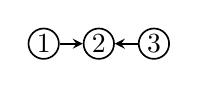
\begin{tikzpicture}[
            > = stealth, % arrow head style
            % shorten > = 1pt, % don't touch arrow head to node
            auto,
            node distance = 7mm, % distance between nodes
            semithick % line style
        ]

        \tikzstyle{every node}=[
        draw = black,
        circle,
        inner sep = 1pt,
        minimum size = 0.1mm
        ]

        \node (1) {$1$};
        \node (2) [right of=1] {$2$};
        \node (3) [right of=2] {$3$};

        \path[->] (1) edge (2);
        \path[->] (3) edge (2);
    \end{tikzpicture}
$$

We may construct a topological ordering of this graph by re-numbering
vertex 3 as vertex 2. We can then draw the graph like this:

$$
    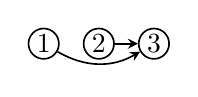
\begin{tikzpicture}[
            > = stealth, % arrow head style
            % shorten > = 1pt, % don't touch arrow head to node
            auto,
            node distance = 7mm, % distance between nodes
            semithick % line style
        ]

        \tikzstyle{every node}=[
        draw = black,
        circle,
        inner sep = 1pt,
        minimum size = 0.1mm
        ]

        \node (1) {$1$};
        \node (2) [right of=1] {$2$};
        \node (3) [right of=2] {$3$};

        \path[->] (1) [bend right] edge (3);
        \path[->] (2) edge (3);
    \end{tikzpicture}
$$

Notice that now the edges all flow in the same direction. If we consider
 the example as an acyclic quiver, we see that arranging the vertices 
 in a topological order means
that $E$ will be an upper triangular matrix; in particular,

$$E = \begin{pmatrix}
    1 & 0 & -1 \\ 0 & 1 & -1 \\ 0 & 0 & 1 \\
\end{pmatrix}
$$

And this can similarly be done with a reversed ordering of the vertices
to obtain a lower triangular $E$. It follows from the definitions that
any topological ordering of a quiver will lead to a $E$ being triangular.
Furthermore, for acyclic quivers, the diagonal entries of $E$ will be 1. 

Therefore, we will use this fact to assume that $E$ is defined as a
triangular matrix with diagonal values of 1
when we use it in examples and calculations. According
to professor Derksen, if such an ordering can be constructed, it will
not change what the eigenvalues of $B$ are \textcolor{red}{TODO: cite}.

\end{example}


\section{The Characteristic Polynomial of $B = -E^T E^{-1}$}

For this section, we assume that $E$ is the Euler matrix of some acyclic quiver,
with the vertices of that quiver numbered such that $E$ is triangular. We consider
the form of the characteristic polynomial of $B = - E^T E^{-1}$.

\begin{proposition}
    The characteristic polynomial of $B$ is reciprocal.
    \begin{proof}
        A \textit{reciprocal polynomial} $P$ is a polynomial such that
        $$P(x) = 0, x \neq 0 \rightarrow P(\frac{1}{x}) = 0$$
        or in other words, a polynomial such that the roots come in reciprocal pairs.

        Let $B = - E^T E^{-1}$ where $E$ has size $n \times n$. Let $P(x) = \det{xI - B}$
        Then 
        $$xI - B = xI + E^T E^{-1}$$
        so 
        $$(xI - B)E = xE + E^T$$
        But since $\det(E) = 1$,
        $$\det(xI - B) = \det(xE + E^T)$$

        We know that since
        $$\det(B) = \pm 1$$
        $x = 0$ is not a root of $\det(xI - B)$,
        and so when
        $$\det(xI - B) = \det(xE + E^T) = 0$$
        we see that 
        $$\det(xE+E^T) = x^n \det(E + \frac{1}{x} E^T)$$
        But for $x \neq 0$,
        $$P(\frac{1}{x}) = \det{E + \frac{1}{x} E^T}$$
        so
        $$P(x) = x^n P(\frac{1}{x})$$
        and therefore by \cite{syz}  $P$ is reciprocal.
    \end{proof}
\end{proposition}

Further research could find more specific restrictions on $\det(xI - B)$.

\section{Roots of $\det(xI - B)$ when $E + E^T$ is positive definite}

Let $B - E^T E^{-1}$ where $E$ is the Euler matrix of some acyclic quiver written
in triangular form. For certain quivers, representation theory can tell us
about the properties of $B$ and and $E$; in particular, the quivers known as
the \textit{simply laced Dynkin diagrams} are well-studied, as they have connections
to many other topics. 

The \textit{simply laced Dynkin diagrams} are $A_n, D_n, E_6, E_7, $ and
    $E_8$; see \cite{dw}. Dynkin diagrams are typically drawn as undirected graphs;
    if we speak of a quiver as being related to a Dynkin diagram, we mean the
    quiver drawn also as an undirected graph. We present the simply laced
    Dynkin diagrams below:

    $$                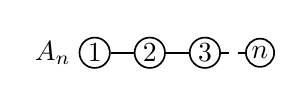
\begin{tikzpicture}[> = stealth, % arrow head style
                % shorten > = 1pt, % don't touch arrow head to node
                auto, node distance = 7mm, % distance between nodes
                semithick % line style
            ]

            \tikzstyle{every node}=[draw = black, circle, inner sep = 1pt,
            minimum size = 1mm]

            \node (1) [label=left:$A_n$] {$1$}; \node (2) [right of=1] {$2$};
            \node (3) [right of=2] {$3$}; \node (4) [right of=3] {$n$};

            \path[-] (1) edge (2); \path[-] (2) edge (3); \path[dashed] (3) edge
            (4);

        \end{tikzpicture}
    $$

    $$                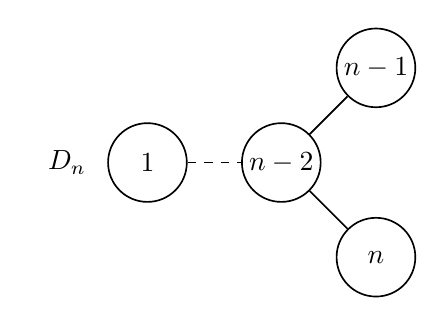
\begin{tikzpicture}[
                > = stealth, % arrow head style
                % shorten > = 1pt, % don't touch arrow head to node
                auto, node distance = 17mm, % distance between nodes
                semithick % line style
            ]

            \tikzstyle{every node}=[draw = black, circle, inner sep = 1pt,
            minimum size = 1cm]

            \node (1) [label=left:$D_n$] {$1$}; \node (2) [right of=1] {$n-2$};
            \node (3) [above right of=2] {$n-1$}; \node (4) [below right of=2]
            {$n$};

            \path[dashed] (1) edge (2); \path[-] (2) edge (3); \path[-] (2) edge
            (4);

        \end{tikzpicture}
    $$

    $$                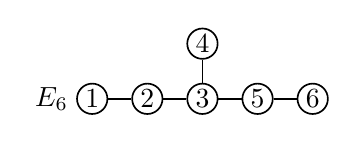
\begin{tikzpicture}[
                > = stealth, % arrow head style
                % shorten > = 1pt, % don't touch arrow head to node
                auto, node distance = 7mm, % distance between nodes
                semithick % line style
            ]

            \tikzstyle{every node}=[draw = black, circle, inner sep = 1pt,
            minimum size = 0.1mm]

            \node (1) [label=left:$E_6$] {$1$}; \node (2) [right of=1] {$2$};
            \node (3) [right of=2] {$3$}; \node (4) [above of=3] {$4$}; \node
            (5) [right of=3] {$5$}; \node (6) [right of=5] {$6$};

            \path[-] (1) edge (2); \path[-] (2) edge (3); \path[-] (3) edge (4);
            \path[-] (3) edge (5); \path[-] (5) edge (6);

        \end{tikzpicture}
    $$

    $$                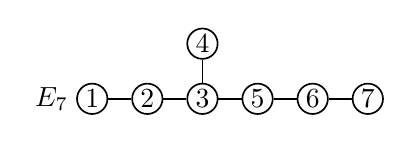
\begin{tikzpicture}[
                > = stealth, % arrow head style
                % shorten > = 1pt, % don't touch arrow head to node
                auto, node distance = 7mm, % distance between nodes
                semithick % line style
            ]

            \tikzstyle{every node}=[draw = black, circle, inner sep = 1pt,
            minimum size = 0.1mm]

            \node (1) [label=left:$E_7$] {$1$}; \node (2) [right of=1] {$2$};
            \node (3) [right of=2] {$3$}; \node (4) [above of=3] {$4$}; \node
            (5) [right of=3] {$5$}; \node (6) [right of=5] {$6$}; \node (7)
            [right of=6] {$7$};

            \path[-] (1) edge (2); \path[-] (2) edge (3); \path[-] (3) edge (4);
            \path[-] (3) edge (5); \path[-] (5) edge (6); \path[-] (6) edge (7);

        \end{tikzpicture}
    $$

    $$                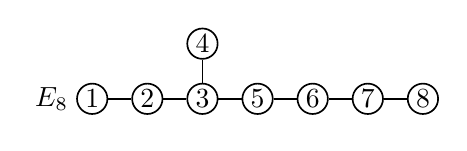
\begin{tikzpicture}[
                > = stealth, % arrow head style
                % shorten > = 1pt, % don't touch arrow head to node
                auto, node distance = 7mm, % distance between nodes
                semithick % line style
            ]

            \tikzstyle{every node}=[draw = black, circle, inner sep = 1pt,
            minimum size = 0.1mm]

            \node (1) [label=left:$E_8$] {$1$}; \node (2) [right of=1] {$2$};
            \node (3) [right of=2] {$3$}; \node (4) [above of=3] {$4$}; \node
            (5) [right of=3] {$5$}; \node (6) [right of=5] {$6$}; \node (7)
            [right of=6] {$7$}; \node (8) [right of=7] {$8$};

            \path[-] (1) edge (2); \path[-] (2) edge (3); \path[-] (3) edge (4);
            \path[-] (3) edge (5); \path[-] (5) edge (6); \path[-] (6) edge (7);
            \path[-] (7) edge (8);

        \end{tikzpicture}
    $$

We know that the roots of $\det(xI - B)$ for these diagrams are all on the unit circle.
We also know that $E + E^T$ is positive definite when the quiver used to define $E$
is a simply laced Dynkin diagram. These two facts are not obviously related, but we
show below that the roots of $\det(xI - B)$ must lie on the unit circle if $E + E^T$
is positive definite.

\begin{proposition} Suppose an acyclic quiver has a
    triangular Euler matrix $E$ and that $E + E^T$ is positive definite.
    Then the solutions to $\det(xI - B)$ lie on the unit circle in the
    complex plane. 
    \begin{proof}
        By assumption, $E + E^T$ is positive
        definite. Consider some $\textbf{v} \in \ker(xE + E^T)$
        where $x$ is a solution of $\det(xE+E^T) = 0$.

        Then $(xE + E^T) \textbf{v} = 0$ so

    $$x E \textbf{v} + E^T \textbf{v} = 0$$

    and therefore $x E \textbf{v} = - E^T \textbf{v}$.

    Furthermore, by taking the conjugate transpose of the above equation we obtain
    $$\textbf{v}^* (xE + E^T)^* = 0$$

    but since $E$ is triangular with integer entries,

    $$\textbf{v}^*(E + xE^T) = 0$$

    so 

    $$\textbf{v}^* E \textbf{v} = - \conj{x} \textbf{v}^* E^T \textbf{v}$$

    But since $x E \textbf{v} = - E^T \textbf{v}$, we can see that

    $$\textbf{v}^* E \textbf{v} = (- \conj{x})(-x \textbf{v}^* E \textbf{v})
    $$

    and therefore
    
    $$\textbf{v}^* E \textbf{v} = |x|^2 \textbf{v}^* E \textbf{v}$$

    Suppose $\textbf{v} E \textbf{v} = 0$. Then 
    $$(\textbf{v} E \textbf{v})^* = 0^*$$
    $$\textbf{v}^* (\textbf{v}^* E)^* = 0$$
    $$\textbf{v}^* E^T \textbf{v} = 0$$

    But $E + E^T$ is positive definite, so 
    $$\textbf{v}^* (E + E^T) \textbf{v} > 0$$
    $$\textbf{v}^* E \textbf{v} + \textbf{v}^* E^T \textbf{v} > 0$$
    $$0 > 0$$

    which is a contradiction. So we know that
    $\textbf{v}^* E \textbf{v} \neq 0$.

    Therefore, since $\textbf{v}^* E \textbf{v} \neq 0$ and 
    $$\textbf{v}^* E \textbf{v} = |x|^2 \textbf{v}^* E \textbf{v}$$
    we see that 
    $$|x|^2 = 1$$
    so $x$ must lie on the unit circle in the complex plane; and since
    $$\det((xI - B)(E)) = \det((xE + E^T) =
    \det(xI - B)\det(E) = \det(xI - B)$$
    we can see that the characteristic polynomial
    of $B = -E^T E^{-1}$ must have roots on the unit circle
    in the complex plane if $E + E^T$ is positive definite.  
    \end{proof}
\end{proposition}

This is not necessarily the case in reverse. Further research could investigate
$E + E^T$ when the roots of $\det(xI - B)$ are known to be on the unit circle.

\textcolor{red}{TODO: Do we mention extended Dynkin here?}

\section{Roots of Subquivers}

In this section, we again consider $B = - E^T E^{-1}$ for some
triangular Euler matrix $E$ for an acyclic quiver. Consider the following
example, created by repeateddly adding a single vertex and edge to a small
quiver:

\tiny
\begin{longtable}[H]{|c|c|c|c|}
    \hline
    \rule{0pt}{3ex}\centered{Quiver} &
    \centered{$\det(xI - B)$} & $M(\det(xI - B))$
    \\
    \hline
    % "Pendulum" example with sequence of subquivers
    \centered{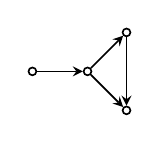
\begin{tikzpicture}[> = stealth, % arrow head style
                % shorten > = 1pt, % don't touch arrow head to node
                auto, node distance = 7mm, % distance between nodes
                semithick % line style
            ]

            \tikzstyle{every node}=[draw = black, circle, inner sep = 1pt,
            minimum size = 0.1mm]

            \node (1) {}; \node (2) [right of=1] {}; \node (3) [above right
                of=2] {}; \node (4) [below right of=2] {};

            \path[->] (1) edge (2); \path[->] (2) edge (4); \path[->] (2) edge
            (3); \path[->] (3) edge (4); \end{tikzpicture}} &
    \centered{$\lambda^{4} - \lambda^{3} - 3\lambda^{2} - \lambda + 1$}
    & \centered{2.3692054071} \\
    \hline

    \centered{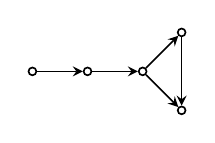
\begin{tikzpicture}[> = stealth, % arrow head style
                % shorten > = 1pt, % don't touch arrow head to node
                auto, node distance = 7mm, % distance between nodes
                semithick % line style
            ]

            \tikzstyle{every node}=[draw = black, circle, inner sep = 1pt,
            minimum size = 0.1mm]

            \node (1) {}; \node (2) [right of=1] {}; \node (3) [above right
                of=2] {}; \node (4) [below right of=2] {}; \node (5) [left of=1]
            {};

            \path[->] (1) edge (2); \path[->] (2) edge (4); \path[->] (2) edge
            (3); \path[->] (3) edge (4); \path[->] (5) edge (1);
        \end{tikzpicture}} &
    \centered{$\lambda^{5} - \lambda^{4} - 3\lambda^{3} - 3\lambda^{2} - \lambda + 1$}
    & \centered{2.618033988770564} \\
    \hline

    \centered{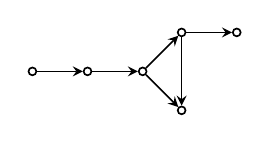
\begin{tikzpicture}[> = stealth, % arrow head style
                % shorten > = 1pt, % don't touch arrow head to node
                auto, node distance = 7mm, % distance between nodes
                semithick % line style
            ]

            \tikzstyle{every node}=[draw = black, circle, inner sep = 1pt,
            minimum size = 0.1mm]

            \node (1) {}; \node (2) [right of=1] {}; \node (3) [above right
                of=2] {}; \node (4) [below right of=2] {}; \node (5) [left of=1]
            {}; \node (6) [right of=3] {};

            \path[->] (1) edge (2); \path[->] (2) edge (4); \path[->] (2) edge
            (3); \path[->] (3) edge (4); \path[->] (5) edge (1); \path[->] (3)
            edge (6);\end{tikzpicture}} &
    \centered{$\lambda^{6} - \lambda^{5} - 5\lambda^{4} - 7\lambda^{3} - 5\lambda^{2} - \lambda + 1$}
    & \centered{3.3014904324145147} \\
    \hline


    \centered{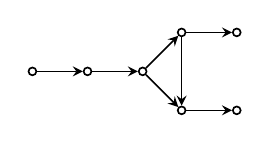
\begin{tikzpicture}[> = stealth, % arrow head style
                % shorten > = 1pt, % don't touch arrow head to node
                auto, node distance = 7mm, % distance between nodes
                semithick % line style
            ]

            \tikzstyle{every node}=[draw = black, circle, inner sep = 1pt,
            minimum size = 0.1mm]

            \node (1) {}; \node (2) [right of=1] {}; \node (3) [above right
                of=2] {}; \node (4) [below right of=2] {}; \node (5) [left of=1]
            {}; \node (6) [right of=3] {}; \node (7) [right of=4] {};

            \path[->] (1) edge (2); \path[->] (2) edge (4); \path[->] (2) edge
            (3); \path[->] (3) edge (4); \path[->] (5) edge (1); \path[->] (3)
            edge (6); \path[->] (4) edge (7); \end{tikzpicture}} &
    \centered{$\lambda^{7} - \lambda^{6} - 7\lambda^{5} - 13\lambda^{4} - 13\lambda^{3} - 7\lambda^{2} - \lambda + 1$}
    & \centered{3.899908930943441} \\
    \hline

    \caption{"Pendulum" quiver sequence and characteristic polynomials of $B$}
    \label{tab:ade}
\end{longtable}
\normalsize

Here, $M(\det(xI - B))$ refers to the \textit{Mahler measure} \cite{m} of the
characteristic polynomial of $B$.
The Mahler measure of a polynomial $P(x) \in \mathbb{Z}[x]$
with integer coefficients
where $$P(x) = a_n \Pi_{k=1}^{n} (x - \alpha_k)$$
is defined as
$$M(P) = |a_d|\Pi_{k=1}^{n}\max\{1, |\alpha_k|\}$$

Notice that the Mahler measure of each quiver is increasing as more edges and vertices
are added. Future work could show that the addition of any edges or
vertices to a quiver cannot lead to a smaller
Mahler measure for $\det(xI - B)$ than the original quiver.

It is not known if there is some $P(x)$ with $M(P) = 1 + \epsilon$
for $\epsilon > 0$. This question is referred to as \textit{Lehmer's Conjecture} or \textit{Lehmer's Question} \cite{m}:
\begin{question} Does there exist some $C > 1$ such that for every polynomial
    $P(x) \in \mathbb{Z}[x]$, $M(P) = 1$ or $M(P) > C$?
\end{question}
Lehmer conjectured that $C \approx 1.1762808$, given by $M(P)$ for $P(x) =
    x^{10} + x^9 - x^7 - x^6 - x^5 - x^4 - x^3 + x + 1$; see \cite{m}.

\section*{Background}

Lehmer first introduced his question in the 1933 paper \textit{Factorization of
    Certain Cyclotomic Functions} \cite{l}. The initial paper was motivated by
an approach for finding large primes \cite{ln}. A lemma of Kronecker implies
that if $M(P) = 1$, then $P$ is a product of powers of $x$ and cyclotomic
polynomials; see \cite{ln}.

Some partial results bounding Mahler measure have been established. Breusch
proved in 1951 that a monic, irreducible, and nonreciprocal polynomial $P$ then
$$M(P) \geq 1.324717\dots$$ which is the real root of $x^3 - x - 1$ \cite{ln}.
Later, in 1979, Dobrowolski showed that for a monic, irreducible, and
non-cyclotomic $P$,
$$M(P) > 1 + c \left(\frac{\log \log d}{\log d}\right)^3$$ for some constant $c$;
see \cite{ln}.

Several computational searches have been carried out in addition to the above
approaches. None have yielded a counterexample to Lehmer's question \cite{m}.
Mossinghoff carried out a search for all polynomials of degree at most 24 with
Mahler measure less than 1.3; while the specific algorithm used applied only to
even degrees, he was able to find 48 such polynomials of degree 22 and 46 of
degree 24 \cite{m}. He was additionally able to use several other algorithms to
extend the search calculations to more degrees, and was able to find a limit
point for measures near 1.309; see \cite{m}.

For more information on the work around Lehmer's question, see the cited works
\textit{Mahler Measure of Polynomials} and \textit{Polynomials with Small Mahler
    Measure}.


\appendix

\section{Examples}

This section contains a table of quivers, their matrices $B$, and plots of the
eigenvalues of $B$ in the complex plane. First, we have the simply laced Dynkin
diagrams.

\setlength\LTleft{-0.75in} \setlength\LTright{-1in}
\tiny
\begin{longtable}[H]{|c|c|c|}
    \hline
    \rule{0pt}{3ex}\centered{Graph}         & \centered{$B = -E^{T} E^{-1}$}                 &
    \centered{Plot of Eigenvalues of
        $B$}
    \\
    \hline
    % Dynkin diagrams
    \centered{
        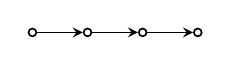
\begin{tikzpicture}[> = stealth, % arrow head style
                % shorten > = 1pt, % don't touch arrow head to node
                auto, node distance = 7mm, % distance between nodes
                semithick % line style
            ]

            \tikzstyle{every node}=[draw = black, circle, inner sep = 1pt,
            minimum size = 0.1mm]

            \node (1) {}; \node (2) [right of=1] {}; \node (3) [right of=2] {};
            \node (4) [right of=3] {};

            \path[->] (1) edge (2); \path[->] (2) edge (3); \path[->] (3) edge
            (4);
        \end{tikzpicture}
    }                                       & \centered{$\begin{pmatrix} -1 & -1
                   & -1 & -1 \\ 1 & 0 & 0 & 0\\ 0 & 1 & 0 & 0\\ 0 & 0 & 1 & 0
                \\\end{pmatrix}$}        &
    \centered{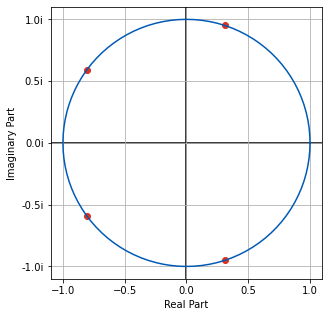
\includegraphics[scale=0.3]{a4.png}}                                                 \\
    \hline
    \centered{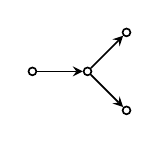
\begin{tikzpicture}[> = stealth, % arrow head style
                % shorten > = 1pt, % don't touch arrow head to node
                auto, node distance = 7mm, % distance between nodes
                semithick % line style
            ]

            \tikzstyle{every node}=[draw = black, circle, inner sep = 1pt,
            minimum size = 0.1mm]

            \node (1) {}; \node (2) [right of=1] {}; \node (3) [above right
                of=2] {}; \node (4) [below right of=2] {};

            \path[->] (1) edge (2); \path[->] (2) edge (4); \path[->] (2) edge
            (3); \end{tikzpicture}}   & \centered{$\begin{pmatrix} -1 & -1 & -1
                   & -1      \\ 1 & 0 & 0 & 0\\ 0 & 1 & 0 & 0\\ 0 & 0 & 1 & 0
                \\\end{pmatrix}$}        &
    \centered{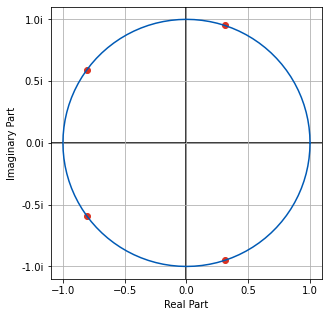
\includegraphics[scale=0.3]{d4.png}}                                             \\
    \hline
    \centered{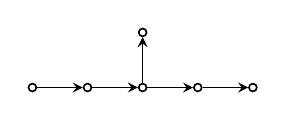
\begin{tikzpicture}[> = stealth, % arrow head style
                % shorten > = 1pt, % don't touch arrow head to node
                auto, node distance = 7mm, % distance between nodes
                semithick % line style
            ]

            \tikzstyle{every node}=[draw = black, circle, inner sep = 1pt,
            minimum size = 0.1mm]

            \node (1) {}; \node (2) [right of=1] {}; \node (3) [right of=2] {};
            \node (4) [above of=3] {}; \node (5) [right of=3] {}; \node (6)
            [right of=5] {};


            \path[->] (1) edge (2); \path[->] (2) edge (3); \path[->] (3) edge
            (4); \path[->] (3) edge (5); \path[->] (5) edge (6);
        \end{tikzpicture}}   & \centered{$\begin{pmatrix} -1 & -1 & -1 & -1
                   & -1 & -1 &              \\ 1 & 0 & 0 & 0 & 0 & 0 & \\ 0 & 1 & 0 & 0
                   & 0  & 0  &              \\
                0  & 0  & 1  & 0  & 1 & 1 & \\ 0 & 0 & 1 & 1 & 0 & 0 & \\ 0 & 0
                   & 0  & 0  & 1  & 0 &     \\
            \end{pmatrix}$}        &
    \centered{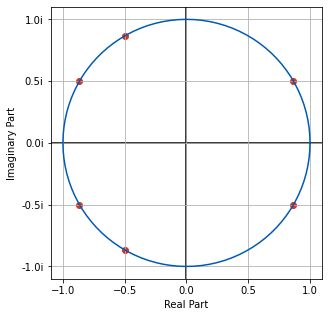
\includegraphics[scale=0.3]{e6.png}}                                             \\
    \hline
    \centered{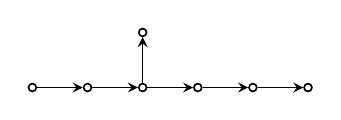
\begin{tikzpicture}[> = stealth, % arrow head style
                % shorten > = 1pt, % don't touch arrow head to node
                auto, node distance = 7mm, % distance between nodes
                semithick % line style
            ]

            \tikzstyle{every node}=[draw = black, circle, inner sep = 1pt,
            minimum size = 0.1mm]

            \node (1) {}; \node (2) [right of=1] {}; \node (3) [right of=2] {};
            \node (4) [above of=3] {}; \node (5) [right of=3] {}; \node (6)
            [right of=5] {}; \node (7) [right of=6] {};


            \path[->] (1) edge (2); \path[->] (2) edge (3); \path[->] (3) edge
            (4); \path[->] (3) edge (5); \path[->] (5) edge (6); \path[->] (6)
            edge (7); \end{tikzpicture}}   & \centered{$\begin{pmatrix} -1 & -1
                   & -1 & -1 & -1 & -1 & -1 & \\ 1 & 0 & 0 & 0 & 0 & 0 & 0 & \\ 0 & 1 &
                0  & 0  & 0  & 0  & 0  &      \\ 0 & 0 & 1 & 0 & 1 & 1 & 1 & \\ 0 &
                0  & 1  & 1  & 0  & 0  & 0  & \\ 0 & 0 & 0 & 0 & 1 & 0 & 0 & \\ 0 &
                0  & 0  & 0  & 0  & 1  & 0  & \\
            \end{pmatrix}$}        &
    \centered{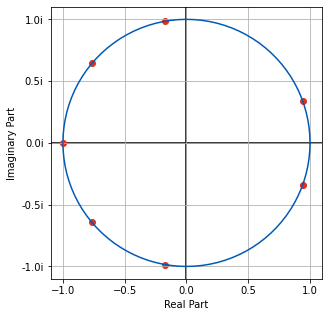
\includegraphics[scale=0.3]{e7.png}}                                             \\
    \hline
    \centered{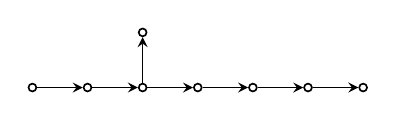
\begin{tikzpicture}[> = stealth, % arrow head style
                % shorten > = 1pt, % don't touch arrow head to node
                auto, node distance = 7mm, % distance between nodes
                semithick % line style
            ]

            \tikzstyle{every node}=[draw = black, circle, inner sep = 1pt,
            minimum size = 0.1mm]

            \node (1) {}; \node (2) [right of=1] {}; \node (3) [right of=2] {};
            \node (4) [above of=3] {}; \node (5) [right of=3] {}; \node (6)
            [right of=5] {}; \node (7) [right of=6] {}; \node (8) [right of=7]
            {};


            \path[->] (1) edge (2); \path[->] (2) edge (3); \path[->] (3) edge
            (4); \path[->] (3) edge (5); \path[->] (5) edge (6); \path[->] (6)
            edge (7); \path[->] (7) edge (8); \end{tikzpicture}}   &
    \centered{$\begin{pmatrix} -1 & -1 & -1 & -1 & -1 & -1 & -1 & -1 &
                \\ 1 & 0 & 0 & 0 & 0 & 0 & 0 & 0 & \\ 0 & 1 & 0 & 0 & 0 & 0 & 0 & 0
                   &                                    \\ 0 & 0 & 1 & 0 & 1 & 1 & 1 &
                1  &                                    \\ 0 & 0 & 1 & 1 & 0 & 0 & 0
                   & 0  &                               \\ 0 & 0 & 0 & 0 & 1 & 0 & 0 &
                0  &                                    \\ 0 & 0 & 0 & 0 & 0 & 1 & 0  & 0  &
                \\ 0 & 0 & 0 & 0 & 0 & 0 & 1  & 0  &                          \\
            \end{pmatrix}$} & \centered{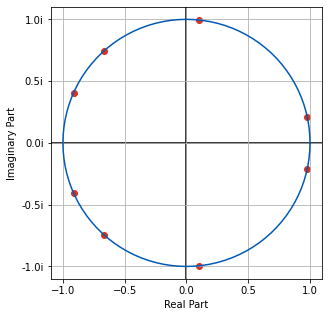
\includegraphics[scale=0.3]{e8.png}}   \\
    \hline
    \caption{\textit{ADE}-quivers and roots of $B$}
    \label{tab:ade}
\end{longtable}

\normalsize
Next we have the extended Dynkin diagrams.

\tiny
\begin{longtable}[H]{|c|c|c|}
    \hline
    \rule{0pt}{3ex}\centered{Graph}         & \centered{$B = -E^{T} E^{-1}$}                     &
    \centered{Plot of Eigenvalues of
        $B$}
    \\
    \hline
    % Extended Dynkin Diagrams
    \centered{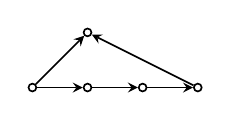
\begin{tikzpicture}[> = stealth, % arrow head style
                % shorten > = 1pt, % don't touch arrow head to node
                auto, node distance = 7mm, % distance between nodes
                semithick % line style
            ]

            \tikzstyle{every node}=[draw = black, circle, inner sep = 1pt,
            minimum size = 0.1mm]

            \node (1) {}; \node (2) [right of=1] {}; \node (3) [right of=2] {};
            \node (4) [right of=3] {}; \node (5) [above of=2] {};


            \path[->] (1) edge (2); \path[->] (2) edge (3); \path[->] (3) edge
            (4); \path[->] (4) edge (5); \path[->] (1) edge (5);
        \end{tikzpicture}}   &

    \centered{$\begin{pmatrix} -1 & -1 & -1 & -1 & -2 & \\ 1 & 0 & 0 & 0 & 1 &
                \\ 0 & 1 & 0 & 0 & 0 & \\ 0 & 0 & 1 & 0 & 0 & \\ 1 & 1 & 1 & 2 &
                2  &                     \\
            \end{pmatrix}$} & \centered{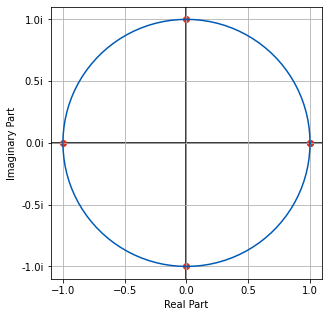
\includegraphics[scale=0.3]{a4_ext.png}}
    \\
    \hline
    \centered{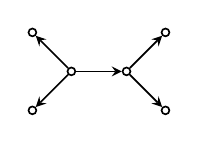
\begin{tikzpicture}[> = stealth, % arrow head style
                % shorten > = 1pt, % don't touch arrow head to node
                auto, node distance = 7mm, % distance between nodes
                semithick % line style
            ]

            \tikzstyle{every node}=[draw = black, circle, inner sep = 1pt,
            minimum size = 0.1mm]

            \node (1) {}; \node (2) [right of=1] {}; \node (3) [above right
                of=2] {}; \node (4) [below right of=2] {}; \node (5) [above left
                of=1] {}; \node (6) [below left of=1] {};


            \path[->] (1) edge (2); \path[->] (2) edge (3); \path[->] (2) edge
            (4); \path[->] (1) edge (5); \path[->] (1) edge (6);
        \end{tikzpicture}}   &

    \centered{$\begin{pmatrix} -1 & -1 & -1 & -1 & -1 & -1 & \\ 1 & 0 & 0 & 0 &
                0  & 0  &                     \\ 0 & 1 & 0 & 0 & 0 & 1 & \\ 0 &
                0  & 1  & 0  & 1  & 0  &      \\ 0 & 0 & 1 & 1  & 0  & 0  & \\ 0
                   & 1  & 1  & 1  & 1  & 0  & \\
            \end{pmatrix}$} & \centered{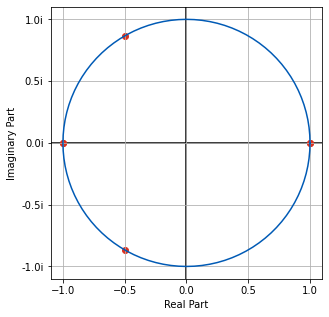
\includegraphics[scale=0.3]{d4_ext.png}}
    \\
    \hline
    \centered{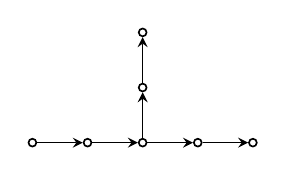
\begin{tikzpicture}[> = stealth, % arrow head style
                % shorten > = 1pt, % don't touch arrow head to node
                auto, node distance = 7mm, % distance between nodes
                semithick % line style
            ]

            \tikzstyle{every node}=[draw = black, circle, inner sep = 1pt,
            minimum size = 0.1mm]

            \node (1) {}; \node (2) [right of=1] {}; \node (3) [right of=2] {};
            \node (4) [above of=3] {}; \node (5) [above of=4] {}; \node (6)
            [right of=3] {}; \node (7) [right of=6] {};


            \path[->] (1) edge (2); \path[->] (2) edge (3); \path[->] (3) edge
            (4); \path[->] (4) edge (5); \path[->] (3) edge (6); \path[->] (6)
            edge (7); \end{tikzpicture}}   &

    \centered{$\begin{pmatrix} -1 & -1 & -1 & -1 & -1 & -1 & -1 & \\ 1 & 0 & 0 &
                0  & 0  & 0  & 0  &                \\ 0 & 1 & 0 & 0 & 0 & 0 & 0
                   &                               \\ 0 & 0 & 1 & 0 & 1 & 1 & 0 &
                \\ 0 & 0  & 1  & 1  & 0  & 0  & 1  &      \\ 0 & 0 & 0  & 0  & 1
                   & 0  & 0  &                     \\ 0 & 0 & 0 & 1 & 0  & 0  & 0  & \\
            \end{pmatrix}$} & \centered{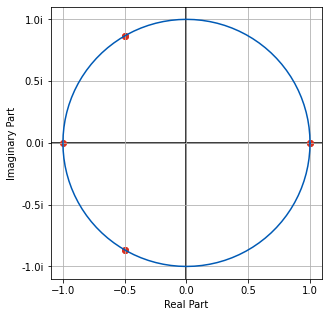
\includegraphics[scale=0.3]{e6_ext.png}}
    \\
    \hline
    \centered{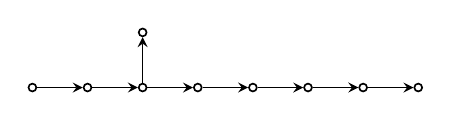
\begin{tikzpicture}[> = stealth, % arrow head style
                % shorten > = 1pt, % don't touch arrow head to node
                auto, node distance = 7mm, % distance between nodes
                semithick % line style
            ]

            \tikzstyle{every node}=[draw = black, circle, inner sep = 1pt,
            minimum size = 0.1mm]

            \node (1) {}; \node (2) [right of=1] {}; \node (3) [right of=2] {};
            \node (4) [above of=3] {}; \node (5) [right of=3] {}; \node (6)
            [right of=5] {}; \node (7) [right of=6] {}; \node (8) [right of=7]
            {}; \node (9) [right of=8] {};


            \path[->] (1) edge (2); \path[->] (2) edge (3); \path[->] (3) edge
            (4); \path[->] (3) edge (5); \path[->] (5) edge (6); \path[->] (6)
            edge (7); \path[->] (7) edge (8); \path[->] (8) edge (9);
        \end{tikzpicture}}   & \centered{$\begin{pmatrix} -1 & -1 & -1 & -1 &
                -1 & -1 & -1 & -1 & -1 &                 \\
                1  & 0  & 0  & 0  & 0  & 0 & 0 & 0 & 0 & \\ 0 & 1 & 0 & 0 &
                0  & 0  & 0  & 0  & 0  &                 \\ 0 & 0 & 1 & 0 & 1 & 1 & 1 & 1 & 1 & \\ 0
                   & 0  & 1  & 1  & 0  & 0 & 0 & 0 & 0 &
                \\ 0 & 0 & 0 & 0 & 1 & 0 & 0 & 0 & 0 & \\ 0 & 0 & 0 & 0 & 0 & 1
                   & 0  & 0  & 0  &                      \\ 0 & 0
                   & 0  & 0  & 0  & 0  & 1 & 0 & 0 &     \\ 0 & 0 & 0 & 0 & 0 & 0 & 0 & 1 &
                0  &                                     \\
            \end{pmatrix}$}            &
    \centered{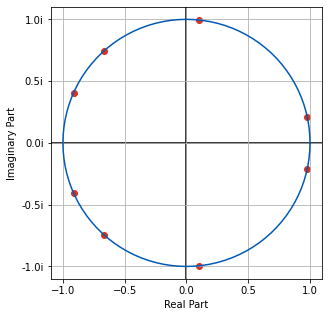
\includegraphics[scale=0.3]{e8.png}}
    \\
    \hline
    \caption{Extended \textit{ADE}-quivers and roots of $B$}
    \label{tab:ade}
\end{longtable}
\normalsize

\section{Source Code}

The source code used to generate examples, graphs, and calculations can
be found at 
\textcolor{blue}{\url{https://github.com/nichols-t/f20-math4020-quiver-matrices}}.
\begin{thebibliography}{99}

    \bibitem{dw} Derksen, H., Weyman, J., {\em An Introduction to Quiver
            Representations\/}, American Mathematical Society, Providence,
    Graduate Studies in Mathematics. {\bf 52} (2017), 1-33.

    \bibitem{m} Mossinghoff, M. J. {\em Polynomials with Small Mahler
            Measure\/}, Mathematics of Computation. {\bf 67} (1998), 1697-1705.

    \bibitem{l} Lehmer, D. H. {\em Factorization of Certain Cyclotomic
            Functions\/}, Annals of Mathematics. {\bf 34} (1933), 461-479.

    \bibitem{ln} Lalin, Matilde N. {\em Mahler Measure of Polynomials\/}
    Postdoctoral Seminar, Mathematical Sciences Research Institute. (2006), 1-2.

    \bibitem{b} Bernstein, Dennis S. {\em Matrix Mathematics \/},
    Princeton University Press. (2005), 44.

    \bibitem{syz} Sun, H., Wang, Y., Zhang, H. X., {\em Polynomials with
    Palindromic and Unimodal Coefficients}, Acta Mathematica Sinica, English
    Series. {\bf 31} (2015), 565-575.

    \bibitem{s} Stankov, Dragan, {\em The number of unimodular roots of some
    reciprocal polynomials}, Reports. Mathematics, {\bf 358} (2020), 159-168.

    \bibitem{sw} Sedgewick, R., Wayne, K., {\em Algorithms: Fourth Edition,
            Part II\/}, Addison-Wesley, Boston. (2014), 574-578.
            
\end{thebibliography}

\end{document}